%% SORI ↔ SoundPLAN 결과 비교 요약(간략판), 단독 컴파일 문서(xelatex 2회)
%% 2026-11-12 개정: 사가정로만 음원(그 밖의 도로 교통량 0)으로 다시 계산, 반사 2·3차를 나란히(‘최종’ 조건 표시 없앰)
%% 수치 출처: sagajeong_only/비교통계.csv, 비교통계_구간.csv(compare.py), 이전 결과 README.md(2026-11-11)
%% 본 문서는 Claude(Anthropic의 AI)를 활용하여 작성하였음.
\documentclass[10pt,a4paper]{article}
\usepackage[a4paper,top=18mm,bottom=18mm,left=18mm,right=18mm]{geometry}
\usepackage{fontspec}
\usepackage{xetexko}
\IfFontExistsTF{Noto Serif CJK KR}{%
  \setmainfont{Noto Serif CJK KR}\setsansfont{Noto Sans CJK KR}%
  \setmainhangulfont{Noto Serif CJK KR}\setsanshangulfont{Noto Sans CJK KR}%
  \setmonohangulfont{Noto Sans CJK KR}[Scale=0.85]}{%
  \setmainfont{Times New Roman}\setsansfont{Apple SD Gothic Neo}%
  \setmainhangulfont{AppleMyungjo}[AutoFakeBold=2.5]\setsanshangulfont{Apple SD Gothic Neo}%
  \setmonohangulfont{Apple SD Gothic Neo}[Scale=0.85]}
\usepackage{booktabs,tabularx,array,graphicx,xcolor}
\usepackage{enumitem,needspace}
\usepackage[hidelinks]{hyperref}
\linespread{1.1}
\setlength{\parindent}{0pt}
\setlength{\parskip}{0.35em}
\setlist{itemsep=0.1em,topsep=0.25em}
\renewcommand{\tablename}{표}
\renewcommand{\figurename}{그림}
\newcolumntype{L}{>{\raggedright\arraybackslash}X}
\newcommand{\f}[1]{\texttt{#1}}
\newcommand{\hl}[1]{\textbf{#1}}

\begin{document}

{\sffamily\Large\bfseries SORI와 SoundPLAN 결과 비교 요약}\\[1mm]
{\sffamily 전농사거리 동쪽 사가정로 구간 · SORI v0.2 · 2026년 11월 12일}

\vspace{2mm}
\fcolorbox{orange!70!black}{orange!8}{\parbox{\dimexpr\linewidth-2\fboxsep-2\fboxrule}{\small
\textbf{읽기 전에.} SoundPLAN 모델(조형찬 작성)의 실제 설정(노면, 반사 차수, 교통량, 신호교차로 보정, 건물 높이)을 받지 못한
\hl{가정 기반 비교}다. 노면과 반사 차수는 SoundPLAN 쪽 값을 모르므로 \hl{반사 2차·3차를 같은 무게로} 함께 적고, 어느 하나를
‘최종’ 조건으로 정하지 않는다. “SoundPLAN과 일치”, “동일 조건 비교”라고 쓰지 않는다.}}

\section*{1. 비교 대상과 방법}
\begin{tabularx}{\linewidth}{@{}p{28mm}L@{}}
\toprule
SoundPLAN 결과 & 2026-11-09 수령. 격자 701점(5 m 간격, 지면 위 2 m), 수음점 2곳(지면 위 1.31 m). 주간 LrD. 모델의 도로는 사가정로 하나 \\
SORI 계산 & SoundPLAN과 \hl{같은 좌표·높이}의 점 수음점으로 계산. RLS-19(음원 + 전파), 서행 30 · 동행 50 km/h, 사가정로 3 + 2차로 차로마다 음원선 \\
음원(이번 개정) & \hl{사가정로만} 현장 실측 교통량(2,540 대/h, 화물차 25.8 \%), \hl{그 밖의 도로 1,223개 객체는 교통량 0}. SoundPLAN 모델에 사가정로만 있는 것과 맞춤 \\
비교 점 & 격자 552점 + 수음점 2곳 = 554점(SoundPLAN 격자 149점은 SORI 건물 안이라 제외 — 두 모델의 건물 자료가 다름) \\
차이 & SORI LrT − SoundPLAN LrD (dB) \\
\bottomrule
\end{tabularx}

\section*{2. 핵심 결과(사가정로만 음원)}
{\small
\begin{tabularx}{\linewidth}{@{}Lrrrrrrr@{}}
\toprule
조건 & 평균 & SD & RMSE & ±2 dB 안 & r & P1 (74.09) & P2 (77.30) \\
\midrule
반사 2차 · 기준 노면(가정) & −0.31 & 3.32 & 3.33 & 61 \% & 0.93 & +0.09 & −0.08 \\
반사 3차 · 기준 노면(가정) & +0.12 & 3.31 & 3.31 & 61 \% & 0.93 & +0.16 & −0.05 \\
반사 3차 · 노면 AC11(SORI 비교 설정) & −2.10 & 3.31 & 3.92 & 39 \% & 0.93 & −2.05 & −2.28 \\
\bottomrule
\end{tabularx}}

{\small 수음점 열의 괄호 안은 SoundPLAN 값(dB), 칸 안은 SORI − SoundPLAN.}
\begin{itemize}
\item \hl{수음점 2곳}은 기준 노면을 가정하면 반사 2·3차 모두 ±0.2 dB 안이다. 반사 2차와 3차의 차이는 0.1 dB 이하.
\item \hl{도로변}(SoundPLAN ≥ 75 dB, 199점)은 평균 −0.2 dB, SD 1.2 dB, ±2 dB 안 89 \%(2·3차 같음).
\item \hl{노면}이 가장 큰 변수다. AC11(승용 −2.7, 화물 −1.9 dB)로 두면 전체가 약 2.2 dB 낮아진다. SoundPLAN 노면은 \hl{미확인}.
\end{itemize}

\begin{figure}[h]\centering
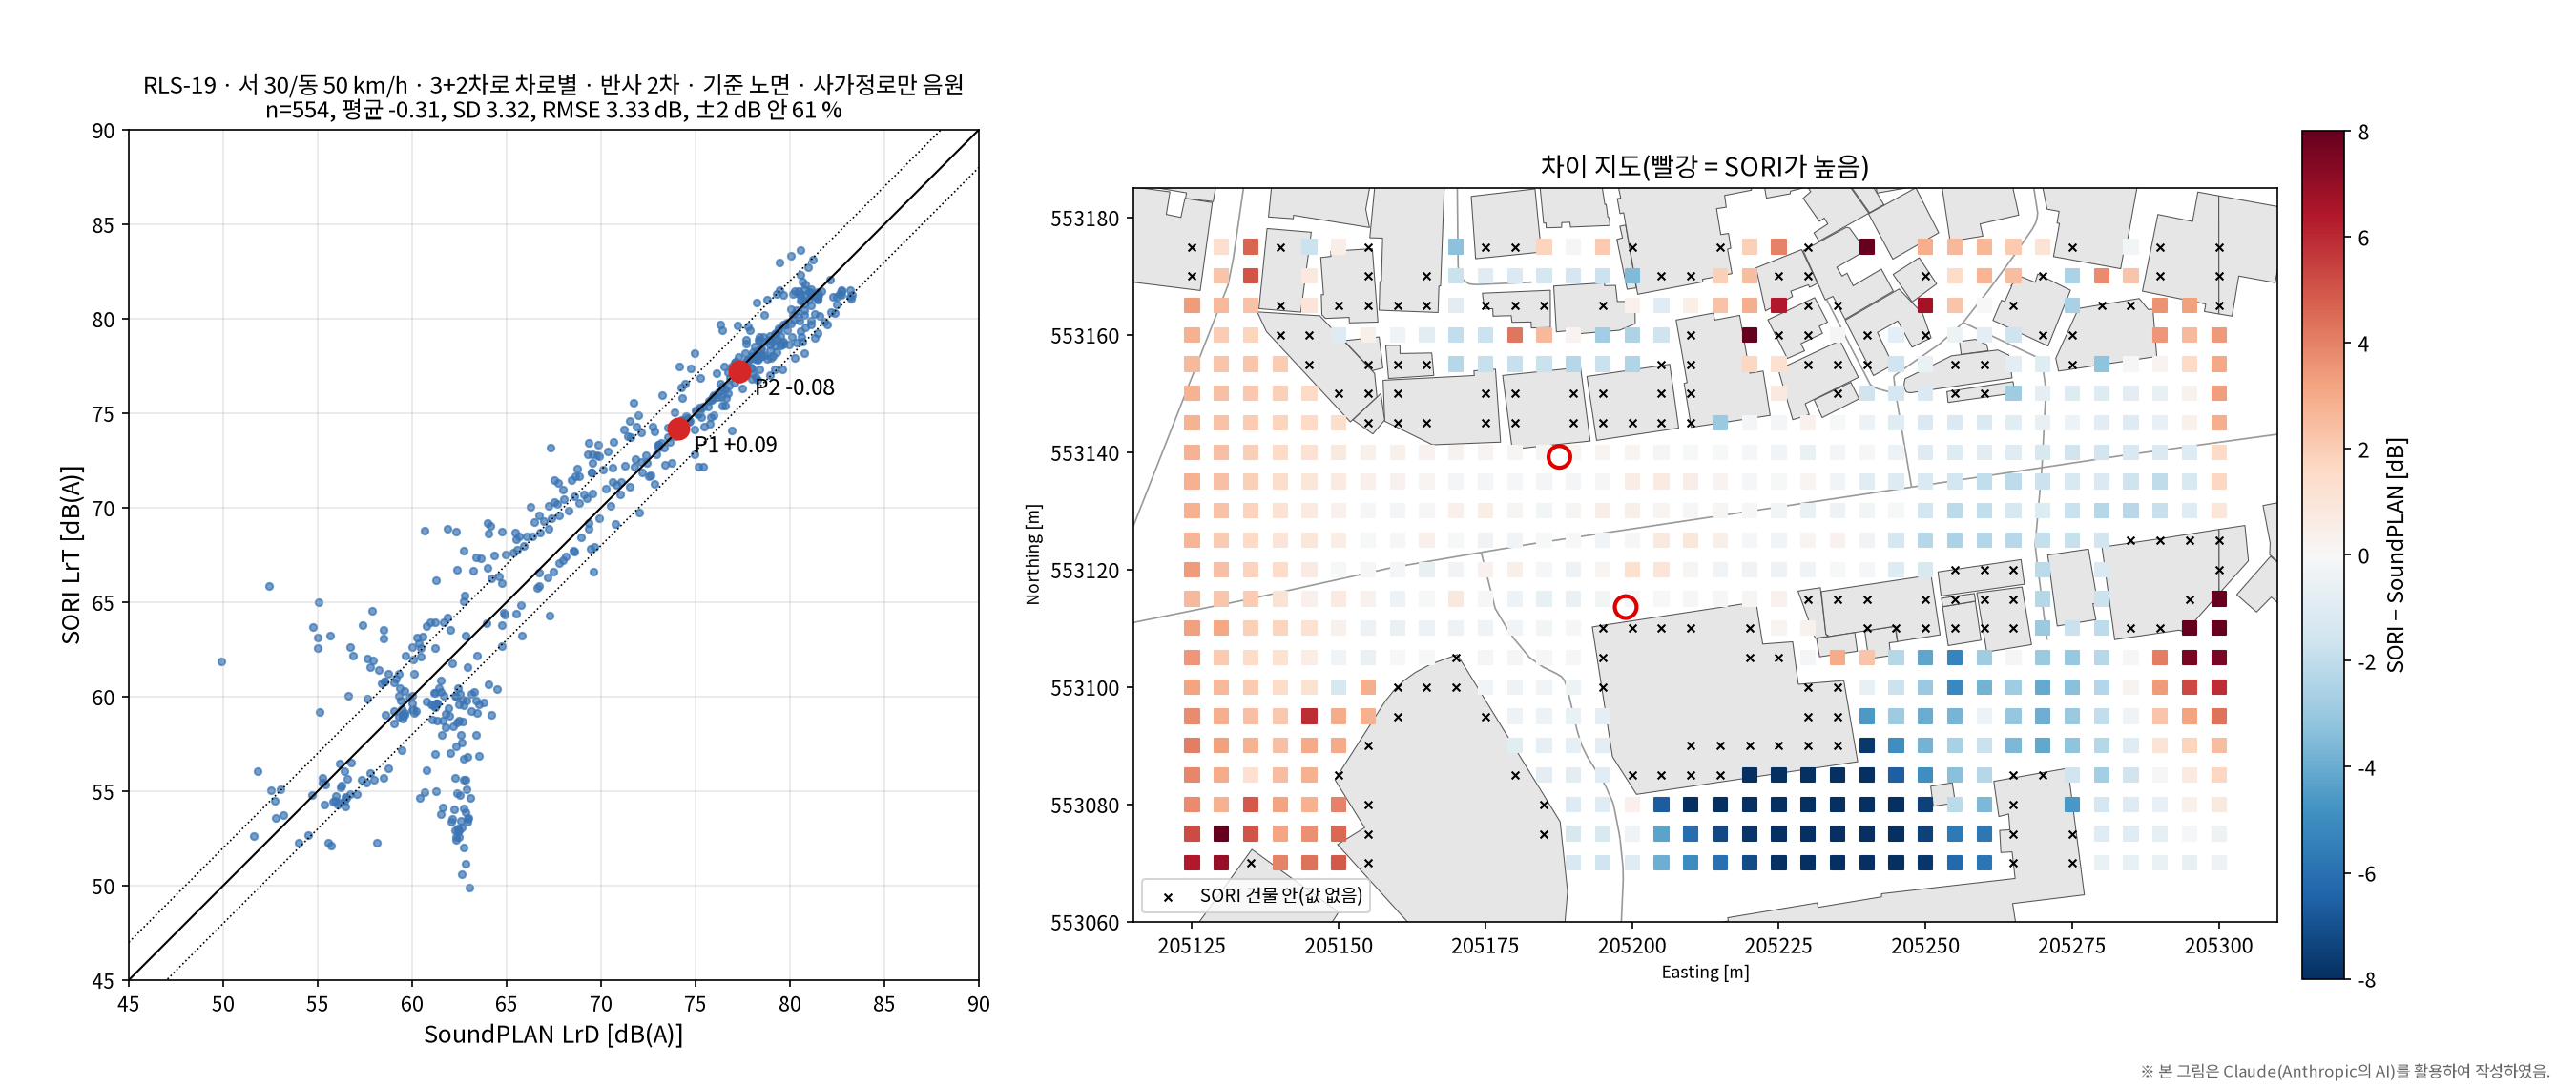
\includegraphics[width=\linewidth]{sagajeong_only/비교_r2_ref.png}\\[1mm]
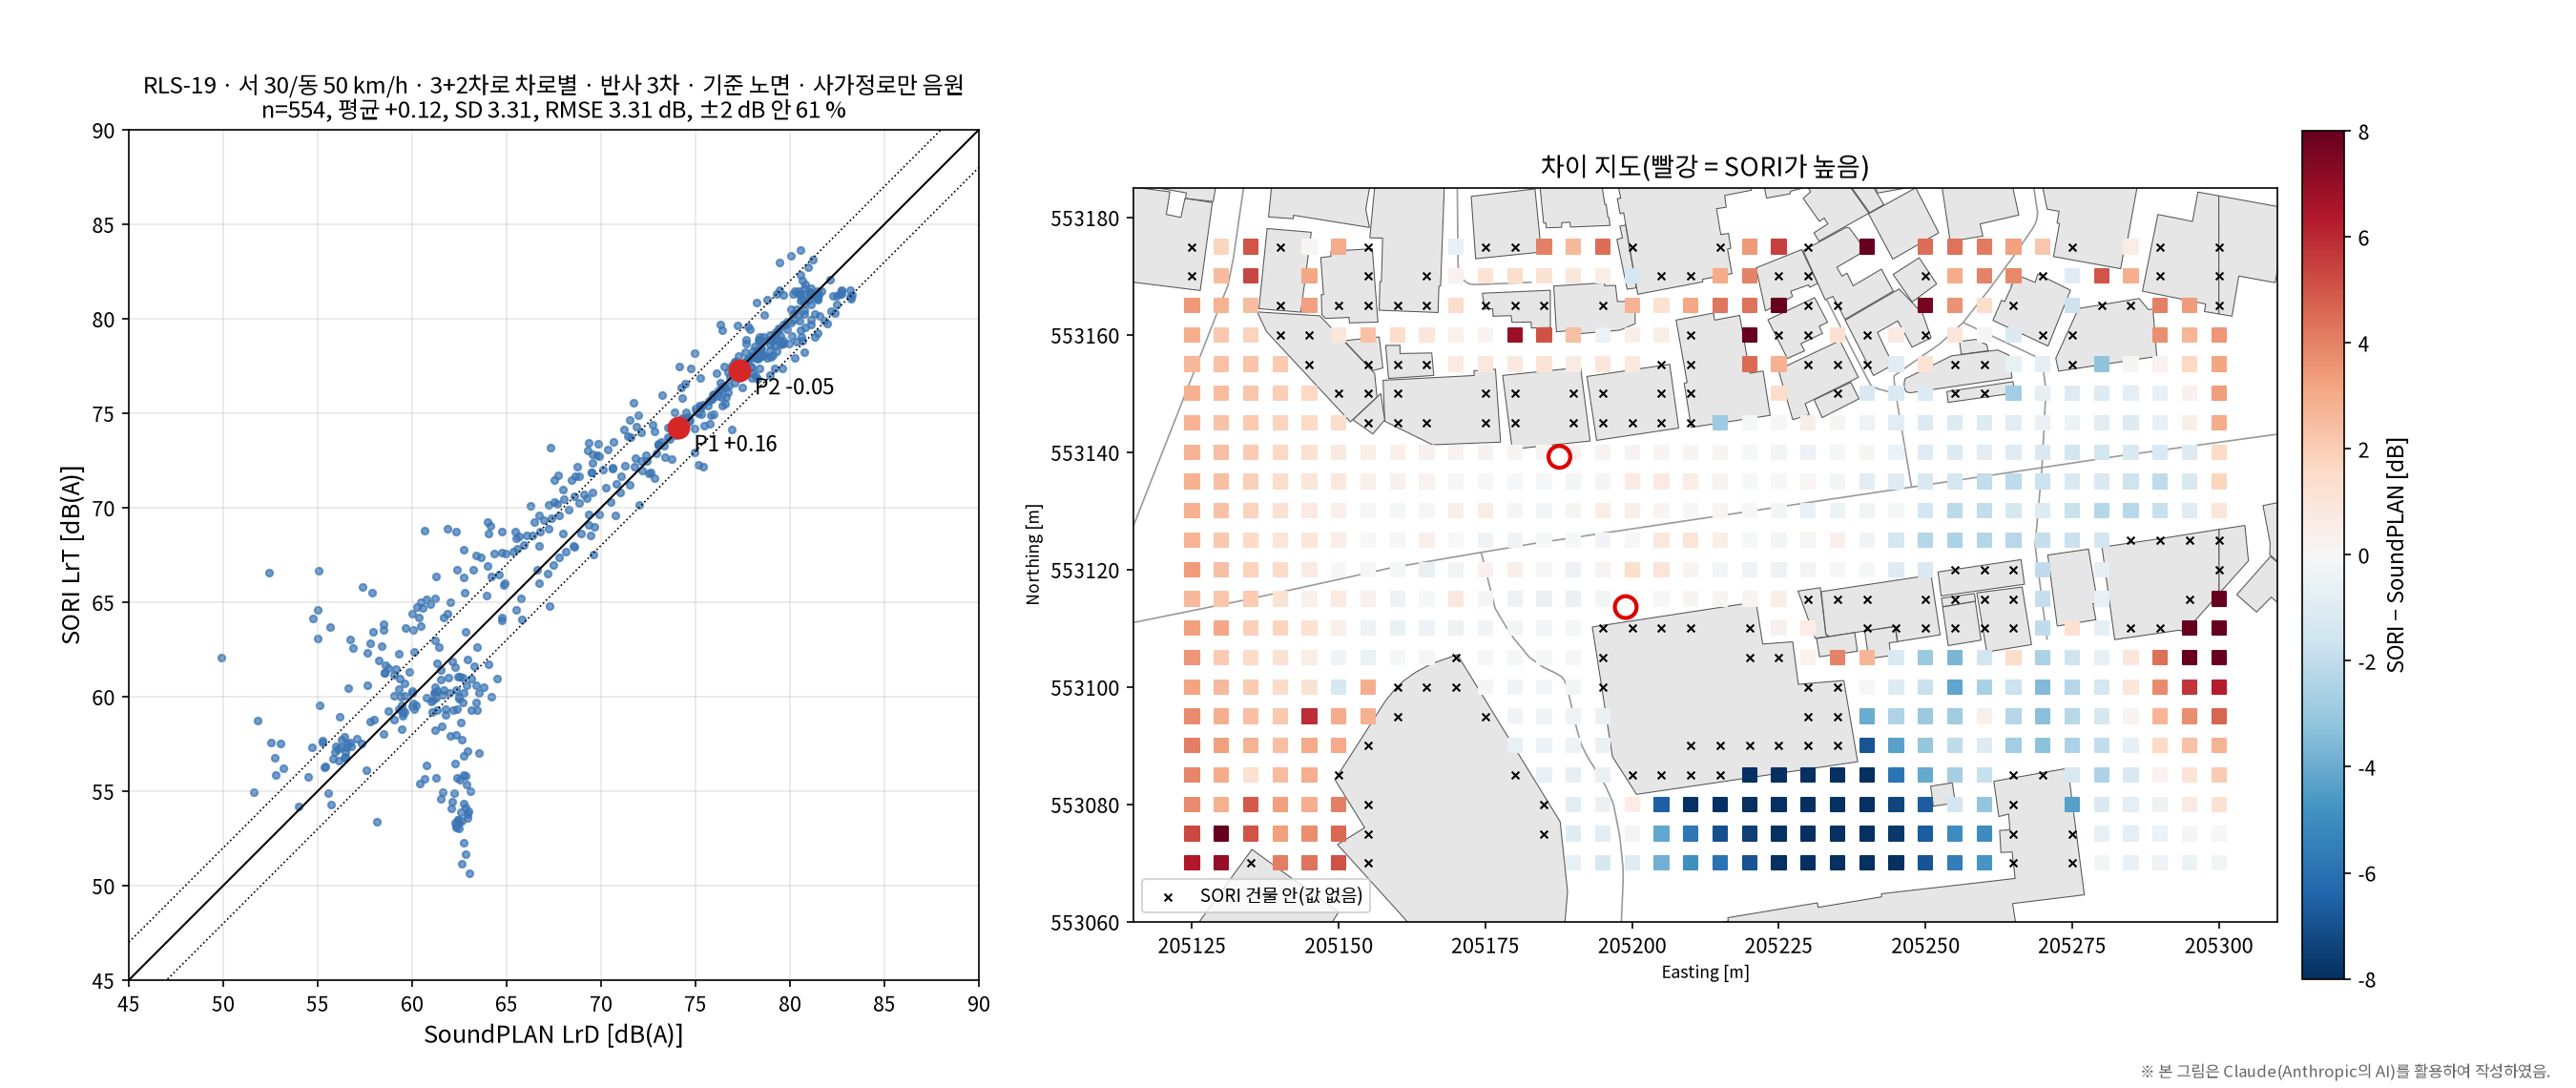
\includegraphics[width=\linewidth]{sagajeong_only/비교_r3_ref.png}
\caption{사가정로만 음원. 위: 반사 2차 · 기준 노면, 아래: 반사 3차 · 기준 노면. 왼쪽 산점도(점선 ±2 dB), 오른쪽 차이 지도(빨강 = SORI가 높음, ○ = 수음점, × = SORI 건물 안)}
\end{figure}

\Needspace{14\baselineskip}
\section*{3. 다른 도로를 뺀 효과(11-11 계산과 비교)}
11-11에는 전농로·답십리로 등 주변 도로(가정 교통량)도 음원이었다. 같은 조건에서 주변 도로만 0으로 바꾼 차이다.

{\small
\begin{tabularx}{\linewidth}{@{}Lrrrrrr@{}}
\toprule
조건 / 음원 & 평균 & SD & RMSE & ±2 dB 안 & P1 & P2 \\
\midrule
반사 2차 · 기준 노면 / 모든 도로 & +0.33 & 3.79 & 3.80 & 57 \% & +0.30 & −0.01 \\
\phantom{반사 2차 · 기준 노면} / \hl{사가정로만} & −0.31 & 3.32 & 3.33 & 61 \% & +0.09 & −0.08 \\
반사 3차 · 기준 노면 / 모든 도로 & +0.75 & 3.79 & 3.86 & 56 \% & +0.36 & +0.03 \\
\phantom{반사 3차 · 기준 노면} / \hl{사가정로만} & +0.12 & 3.31 & 3.31 & 61 \% & +0.16 & −0.05 \\
반사 3차 · AC11 / 모든 도로 & −1.49 & 3.77 & 4.05 & 34 \% & −1.86 & −2.21 \\
\phantom{반사 3차 · AC11} / \hl{사가정로만} & −2.10 & 3.31 & 3.92 & 39 \% & −2.05 & −2.28 \\
\bottomrule
\end{tabularx}}

\begin{itemize}
\item 주변 도로를 빼자 흩어짐(SD)이 3.8 → 3.3 dB로 줄고 상관 r이 0.91 → 0.93으로 올랐다. 수음점 값은 0.1–0.2 dB만 바뀌었다(사가정로가 지배적).
\item 서쪽 구역(x < 205160, 129점)의 평균 차이는 기준 노면에서 +4.1 → +2.2 dB(2차), +4.2 → +2.3 dB(3차)로 줄었다. 남은 +2 dB는 교차로 쪽 사가정로 음원 범위나 신호교차로 보정 D\textsubscript{K} 차이로 보이며 \hl{미확인}.
\end{itemize}

\section*{4. 레벨 구간별 차이(사가정로만, 기준 노면, 격자 552점)}
{\small
\begin{tabularx}{\linewidth}{@{}Lrrrrrrrr@{}}
\toprule
 & & \multicolumn{3}{c}{반사 2차} & & \multicolumn{3}{c}{반사 3차} \\
\cmidrule(lr){3-5}\cmidrule(lr){7-9}
SoundPLAN LrD & n & 평균 & SD & ±2 dB 안 & & 평균 & SD & ±2 dB 안 \\
\midrule
≥ 75 dB (도로변) & 199 & −0.21 & 1.17 & 89 \% & & −0.18 & 1.16 & 89 \% \\
70–75 & 67 & +0.68 & 1.40 & 75 \% & & +0.77 & 1.33 & 76 \% \\
65–70 & 64 & +1.44 & 1.97 & 42 \% & & +1.64 & 1.77 & 42 \% \\
60–65 (건물 뒤가 많음) & 137 & −2.69 & 4.80 & 25 \% & & −2.05 & 4.84 & 28 \% \\
< 60 & 85 & +1.19 & 3.57 & 55 \% & & +2.63 & 3.28 & 52 \% \\
\bottomrule
\end{tabularx}}

도로변은 가깝고 건물 뒤·먼 점은 흩어짐이 크다(구간 안 상관 r: 도로변 0.85, 60–65 dB 구간 0.13–0.16). 전체 r = 0.93은 도로변과 뒤편의 레벨 차이가 만든 값이며 점별 일치를 뜻하지 않는다. 남측 큰 건물 뒤(차이 지도 아래쪽 파랑)는 SORI가 6 dB 이상 낮다 — 건물 자료(범위·높이)와 차폐 조건 차이로 보이며 \hl{미확인}.

\section*{5. 한계와 다음 단계}
\begin{itemize}
\item 이 비교는 SORI의 \hl{RLS-19 음원 + RLS-19 전파}를 본 것이다. SORI 기본 조합(RLS-19 음원 + ISO 9613-2 전파)을 검증한 것이 아니다. SORI 기본 반사 차수는 3차 그대로다.
\item SORI는 신호교차로 보정 D\textsubscript{K}와 다중반사 가산 D\textsubscript{refl}을 넣었다. SoundPLAN 사용 여부는 미확인.
\item 격자점은 5 m 간격이라 서로 독립이 아니다. SD·RMSE는 구역별 차이의 크기로 읽는다.
\item 현장 측정 LAeq(지점1 68.6, 지점2 69.1 dB)보다 SoundPLAN도 약 5.5·8 dB 높다. “SoundPLAN과 가깝다”가 “현장 예측이 맞다”를 뜻하지 않는다.
\item \hl{SoundPLAN 쪽에서 받아야 할 것}: 노면 종류, 반사 차수·반사 손실, 교통량·화물차 비율·속도, 사가정로 음원 범위(교차로 쪽 끝), 신호교차로 지정, 다중반사 가산 사용 여부, 건물 높이 산정, 지형, 도로 방출표(L\textsubscript{W}′).
\end{itemize}

\vspace{2mm}
{\footnotesize 다시 계산: \f{sagajeong\_only/<조건>/config.yaml}(교통량 \f{sagajeong\_only/traffic.csv}), 통계·그림 \f{sagajeong\_only/compare.py}. 이전 기록 \f{README.md}. ※ 본 문서는 Claude(Anthropic의 AI)를 활용하여 작성하였음. 계산 결과의 검토·검증 책임은 사용자에게 있음.}

\end{document}
